\documentclass[10pt]{extarticle}

\usepackage[margin=1.8cm]{geometry}
\usepackage{xcolor}
\usepackage{amsmath,amssymb}
\usepackage{tcolorbox}
\usepackage{enumitem}
\usepackage{graphicx}
\usepackage[
  colorlinks=true,
  linkcolor=blue!50!black,
  citecolor=green!35!black,
  urlcolor=blue!60!black
]{hyperref}

\renewcommand{\sectionautorefname}{Section}
\renewcommand{\subsectionautorefname}{Section}
\renewcommand{\figureautorefname}{Figure}
\renewcommand{\tableautorefname}{Table}
\renewcommand{\equationautorefname}{Equation}

\setlist[enumerate]{
  leftmargin=3.5em,
  itemsep=1pt,
  topsep=3pt,
  parsep=0pt,
  partopsep=0pt
}

\title{Tanaka Certificates}
% \author{}
\date{\today}

\tcbset{
  notebox/.style={
    boxrule=0.3pt,
    arc=0.5mm,
    left=2mm,
    right=2mm,
    top=1.5mm,
    bottom=1.5mm,
    fonttitle=\bfseries
  }
}

\newtcolorbox{setup}{
  notebox,
  title=Setup,
  colback=blue!2,
  colbacktitle=blue!12,
  colframe=blue!25!black,
  coltitle=blue!45!black
}

\newtcolorbox{hypothesis}{
  notebox,
  title=Hypothesis,
  colback=yellow!3,
  colbacktitle=yellow!18,
  colframe=yellow!45!black,
  coltitle=yellow!25!black
}

\newtcolorbox{fact}{
  notebox,
  title=Fact,
  colback=green!2,
  colbacktitle=green!12,
  colframe=green!25!black,
  coltitle=green!30!black
}

\newtcolorbox{sidenote}{
  notebox,
  title=Sidenote,
  colback=gray!3,
  colbacktitle=gray!12,
  colframe=gray!35!black,
  coltitle=gray!45!black
}

\begin{document}

\maketitle

\begin{abstract}
  In these notes, I am building up the intuition and theory behind supermartingale certificates, with relaxed assumptions on the certificate function $V$. In particular, it is explored what happens when $V$ is not twice continously-differentiable, but instead piecewise twice continuously-differentiable.
\end{abstract}

\tableofcontents
\clearpage

\section{Piecewise linear certificates in dimension one}
\label{sec:piecewise-linear}

Consider the following setup:

\begin{setup}
Let:
\begin{enumerate}
    \item $dX_t = f(X_t) dt + g(X_t) dW_t$ be a one-dimensional SDE
    \item $V(x)$ be a piecewise linear function such that $V(x) = a_i x + b_i$, where $x \in \left( x_i, x_{i+1} \right)$.
    \item $V(x)$ is continuous at breakpoints: $V(x_i^+)=V(x_i^-) = V(x_i)$
    \item as a consequence, $V'_{-}(x_i) = a_{i-1}$, $V'_{+}(x_i) = a_i$
\end{enumerate}

\end{setup}

Now we will consider what conditions on $V$ are sufficient to guarantee that $V(X_t)$ is a supermartingale.

\begin{hypothesis}
Does concavity of $V(x)$ (along with an interior / drift term condition) guarantee that $V(X_t)$ is a supermartingale?
\end{hypothesis}

To answer this, let's apply the Itô-Tanaka formula to $V(X_t)$:
\begin{align}
    V(X_t) = V(X_0) + &\int_0^t V'(X_s) f(X_s) ds \\
        + &\int_0^t V'(X_s) g(X_s) dW_s \\
        + \frac{1}{2} &\sum_{i=1}^{n-1} \left( V'_{+}(x_i) - V'_{-}(x_i) \right) L_t^{x_i}(X) \\
\end{align}

We will focus on these terms: 

\begin{enumerate}
  \item $D_t = \int_0^t V'(X_s) f(X_s) ds$, the drift term
  \item $M_t = \int_0^t V'(X_s) g(X_s) dW_s$, the diffusion term (stochastic integral)
  \item $K_t = \frac{1}{2} \sum_{i=1}^{n-1} \left( V'_{+}(x_i) - V'_{-}(x_i) \right) L_t^{x_i}(X)$, the kink term
\end{enumerate}

we need to prove that $D_t + M_t + K_t$ is a supermartingale.

Some natural assumptions, which are sufficient to guarantee that $V(X_t)$ is a supermartingale, are the following:
\begin{enumerate}
  \item $f(x) V'(x) \leq 0$ for all $x \in (x_i, x_{i+1})$. This is because of the following:
  
  \begin{fact}
  \label{fact:nonpositive-drift-supermartingale}
  If $f(X) V'(X) \leq 0$, then the drift term $D_t$ is a supermartingale. \\
  \linebreak
  \textbf{Proof:} We want to prove $\mathbb{E}[D_t | \mathcal{F}_s] \leq D_s$ for $s \leq t$.
  \begin{align}
    \mathbb{E}[D_t | \mathcal{F}_s] &= \mathbb{E}\left[\int_0^t V'(X_u) f(X_u) du \Big| \mathcal{F}_s\right] \\
    &= \int_0^s V'(X_u) f(X_u) du + \mathbb{E}\left[\int_s^t V'(X_u) f(X_u) du \Big| \mathcal{F}_s\right] \\
    &\leq D_s + 0 = D_s
  \end{align}
  \end{fact}

  \item $M_t$ is a martingale. Assuming $V(x)$ has finitely many pieces
  (as is the case for a neural network with ReLU activation functions), it is enough
  to impose a square-integrability condition on $g(x)$\footnote{For example,
  $\mathbb{E}\!\left[\int_0^t g(X_s)^2\,ds\right]<\infty$.}
  
  \item $V'_{+}(x_i) - V'_{-}(x_i) \leq 0 \iff a_{i-1} \geq a_i$, i.e. the \textbf{concavity condition}. This is because of the following:
  \begin{fact}
    If $V'_{+}(x_i) - V'_{-}(x_i) \leq 0$ and $L_t^{x_i}(X) \geq 0$, then the kink term $K_t$ is a supermartingale. \\
    \linebreak
    \textbf{Proof:} We want to prove $\mathbb{E}[K_t | \mathcal{F}_s] \leq K_s$ for $s \leq t$.
    \begin{align}
      \mathbb{E}[K_t | \mathcal{F}_s] &= \mathbb{E}\left[\frac{1}{2} \sum_{i=1}^{n-1} \left( V'_{+}(x_i) - V'_{
-}(x_i) \right) L_t^{x_i}(X) \Big| \mathcal{F}_s\right] \\
      &= \frac{1}{2} \sum_{i=1}^{n-1} \left( V'_{+}(x_i) - V'_{-}(x_i) \right) \mathbb{E}\left[L_t^{x_i}(X) | \mathcal{F}_s\right] \\
      &\leq \frac{1}{2} \sum_{i=1}^{n-1} \left( V'_{+}(x_i) - V'_{-}(x_i) \right) L_s^{x_i}(X) = K_s
    \end{align}
    Note that the inequality follows from the fact that $L_t^{x_i}(X)$ is non-decreasing in $t$, hence $\mathbb{E}\left[L_t^{x_i}(X) | \mathcal{F}_s\right] \geq \mathbb{E}\left[L_s^{x_i}(X) | \mathcal{F}_s\right] = L_s^{x_i}(X)$.
  \end{fact}

\end{enumerate}

We will consider what happens in different practical cases to these terms, including: 
\begin{enumerate}
  \item A simple one-dimensional SDE with a piecewise linear certificate.
  \item A pendulum with a stochastic torque, and $X_t$ measuring the angle of the pendulum.
  \item A network $b$ black and $w$ white nodes, with given transition probabilities, and $X_t$ measuring the amount of mass in the white nodes. 
\end{enumerate}
to ensure our assumptions are reasonable.

\subsection{Proof of the supermartingale property}

First, let's note the following:

\begin{fact}
  The sum of a martingale and a supermartingale is a supermartingale. \\
  \linebreak
  \textbf{Proof}: By definition, given a martingale $M_t$ and a supermartingale $S_t$, for $r < t$ we have 
  $\mathbb{E}[M_t | \mathcal{F}_r] = M_r$ and 
  $\mathbb{E}[M_t | \mathcal{F}_r] \leq S_r$. Then, for $r < t$:
  \begin{align}
    \mathbb{E}[M_t + S_t | \mathcal{F}_r] &= \mathbb{E}[M_t | \mathcal{F}_r] + \mathbb{E}[S_t | \mathcal{F}_r] \\
    &= M_r + \mathbb{E}[S_t | \mathcal{F}_r] \\
    &\leq M_r + S_r = (M + S)_r
  \end{align}
\
hence $M_t + S_t$ is a supermartingale.

\end{fact}

The drift term $D_t$ is a supermartingale by assumption 1. The kink term $K_t$ is a supermartingale by assumption 3. The stochastic integral $M_t$ is a martingale by assumption 2. Therefore, the sum of these three terms is a supermartingale (as a consequence of the previous fact), and hence $V(X_t)$ is a supermartingale.


\section{Piecewise $\mathcal{C}^2$ certificates in dimension one}

The setup is pretty similiar, with the exception that $V$ is now piecewise $\mathcal{C}^2$ instead of piecewise linear. 

\begin{setup}
Let:
\begin{enumerate}
    \item $dX_t = f(X_t) dt + g(X_t) dW_t$ be a one-dimensional SDE.
    \item $V(x)$ be a piecewise $\mathcal{C}^2$ function such that $V(x) \in \mathcal{C}^2$, where $x \in \left( x_i, x_{i+1} \right)$.
    \item $V(x)$ is continuous at breakpoints: $V(x_i^+)=V(x_i^-) = V(x_i)$.
\end{enumerate}

\end{setup}

We will again consider what conditions on $V$ are sufficient to guarantee that $V(X_t)$ is a supermartingale. Again, the natural hypothesis is:

\begin{hypothesis}
Does concavity of $V(x)$ (along with an interior / drift term condition) guarantee that $V(X_t)$ is a supermartingale?
\end{hypothesis}

We apply the Itô-Tanaka formula to $V(X_t)$, and we get similiar terms, with the addition of
\begin{equation}
  C_t = \frac{1}{2} \int_{0}^{t} V''(X_s) g^2(X_s) ds
\end{equation}

Since the integral in the $C_t$ term is over the same intervals as the $D_t$ term, we can combine them to recover the generator / Lie derivative term:
\begin{equation}
  D_t + C_t = \int_{0}^{t} \left( V'(X_s) f(X_s) + \frac{1}{2} V''(X_s) g^2(X_s) \right) ds = \int_{0}^{t} \mathcal{L} V(X_s) ds
\end{equation}

The proof that $V(X_t)$ is a supermartingale is similiar to the piecewise linear case, but now we need to impose the condition:
\begin{equation}
  \mathcal{L} V(x) = V'(x) f(x) + \frac{1}{2} V''(x) g^2(x) \leq 0
\end{equation}

\newpage


\section{Studying piecewise certificates on concrete one-dimensional examples}

Some useful examples to study are given in Tables~\ref{tab:kink-examples}
and~\ref{tab:curvature-examples}.

\begin{table}[t]
\centering
\caption{Piecewise linear certificates examples.}
\label{tab:kink-examples}
\begin{tabular}{lllll}
\hline
SDE & $V(x)$ & $D_t$ & $M_t$ & $K_t$ \\
\hline
$dX_t=dW_t$
&
$-|x|$
&
$0$
&
$\displaystyle \int_0^t -\operatorname{sgn}(X_s)\,dW_s$
&
$\displaystyle -L_t^0(X)$
\\[1.1em]

% $dX_t=dW_t$
% &
% $|x|$
% &
% $0$
% &
% $\displaystyle \int_0^t \operatorname{sgn}(X_s)\,dW_s$
% &
% $\displaystyle L_t^0(X)$
% \\[1.1em]

$dX_t=-X_t\,dt$
&
$|x|$
&
$\displaystyle -\int_0^t |X_s|\,ds$
&
$0$
&
$0$
\\
\hline
\end{tabular}
\end{table}

\begin{table}[t]
\centering
\caption{Piecewise $\mathcal{C}^2$ certificates examples.}
\label{tab:curvature-examples}
\resizebox{\textwidth}{!}{%
\begin{tabular}{llllll}
\hline
SDE & $V(x)$ & $D_t$ & $M_t$ & $C_t$ & $K_t$ \\
\hline
$dX_t=-\lambda X_t\,dt+\sigma\,dW_t$
&
$x^2$
&
$\displaystyle -2\lambda \int_0^t X_s^2\,ds$
&
$\displaystyle \int_0^t 2\sigma X_s\,dW_s$
&
$\displaystyle \sigma^2 t$
&
$0$
\\[1.1em]

$dX_t=dt+\sqrt{2}\,dW_t$
&
$\displaystyle x-\frac{x^2}{2}$
&
$\displaystyle \int_0^t (1-X_s)\,ds$
&
$\displaystyle \int_0^t (1-X_s)\sqrt{2}\,dW_s$
&
$\displaystyle -t$
&
$0$
\\[1.1em]

$dX_t=dW_t$
&
$\displaystyle
\begin{cases}
-\frac12 x^2, & x<0,\\
-x, & x\ge 0
\end{cases}$
&
$0$
&
$\displaystyle \int_0^t V'(X_s)\,dW_s$
&
$\displaystyle -\frac12\int_0^t \mathbf 1_{\{X_s<0\}}\,ds$
&
$\displaystyle -\frac12 L_t^0(X)$
\\
\hline
\end{tabular}%
}
\end{table}

\subsection{Ornstein--Uhlenbeck process in three parameter regimes}

Consider the Ornstein--Uhlenbeck process
\[
  dX_t=-\lambda X_t\,dt+\sigma\,dW_t
\]
with the quadratic certificate $V(x)=x^2$. Its generator is
\[
  \mathcal LV(x)=-2\lambda x^2+\sigma^2
  =-2\lambda\left(x^2-\frac{\sigma^2}{2\lambda}\right).
\]
Consequently, if
\[
  r=\frac{\sigma}{\sqrt{2\lambda}},
\]
then the generator is negative for $|x|>r$, zero for $|x|=r$, and positive
for $|x|<r$. The decomposition is
\[
  X_t^2-X_0^2
  =\underbrace{-2\lambda\int_0^t X_s^2\,ds}_{D_t}
  +\underbrace{2\sigma\int_0^t X_s\,dW_s}_{M_t}
  +\underbrace{\sigma^2t}_{C_t},
\]
with $K_t=0$.

Figure~\ref{fig:ou-terms} fixes $\lambda=1$ and $X_0=1$, and uses
$r=0.5$, $r=1$, and $r=1.5$. These choices make the initial generator
negative, zero, and positive, respectively. Moreover,
\[
  \mathbb E[X_t^2]
  =r^2+(X_0^2-r^2)e^{-2\lambda t},
\]
so the expected generator retains the corresponding sign. In the middle
case, $X_t^2$ is constant in expectation, but it is not a martingale: the
pointwise generator vanishes only when $|X_t|=r$.

The stochastic integral $M_t$ need not visibly oscillate on every individual
sample path; the martingale statement is instead that its conditional drift
is zero. Figure~\ref{fig:ou-terms} therefore plots Monte Carlo expectations.
The mean of $M_t$ remains statistically consistent with zero, while $D_t$ and
$C_t$ determine whether $\mathbb E[X_t^2-X_0^2]$ decreases, remains zero, or
increases.

\begin{figure}[htbp]
  \centering
  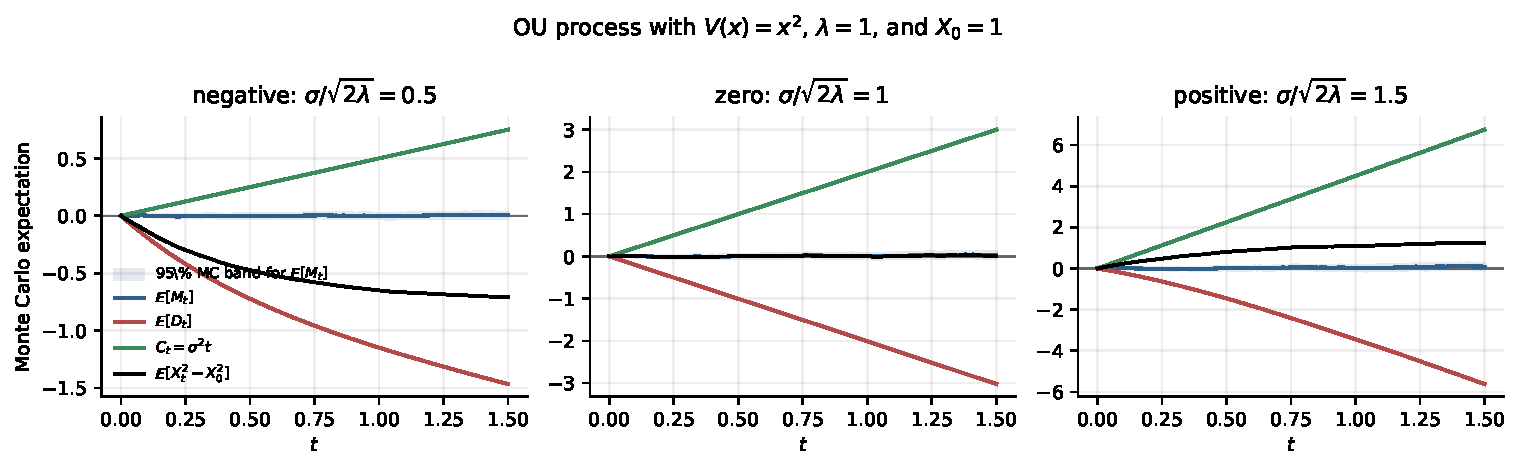
\includegraphics[width=\textwidth]{figures/ou_generator_three_cases.pdf}
  \caption{Monte Carlo expectations from $8000$ Ornstein--Uhlenbeck paths for
  $V(x)=x^2$. The three columns use
  $\sigma/\sqrt{2\lambda}=0.5,1,1.5$. The shaded region is a pointwise
  approximate 95\% Monte Carlo band for $\mathbb E[M_t]$.}
  \label{fig:ou-terms}
\end{figure}

\subsection{Failure of piecewise linearity and success of curvature}

For $f=1$ and $g=\sqrt{2}$ on $[0,1]$, consider a case where want to find a certificate $V$ such that $V(0) = 0$ and $V(1) = 1$.

% the increasing linear candidate
% $V_{\mathrm{PL}}(x)=x$ has
% \[
%   \mathcal{L}V_{\mathrm{PL}}(x)=1>0.
% \]
% More generally, an increasing piecewise-linear certificate must have positive
% slope on some open interval; on that interval its curvature vanishes and
% $\mathcal{L}V=V'>0$. 

A smooth candidate could be:
\[
  V_{\mathcal C^2}(x)=x-\frac{x^2}{2},
\]
the curvature contribution compensates for the positive drift:
\[
  \mathcal{L}V_{\mathcal C^2}(x)
  =(1-x)+\frac12(-1)(2)=-x\leq0.
\]

and indeed $V_{\mathcal C^2}$ is a valid supermartingale certificate.

On the other hand, let's assume $V$ is piecewise linear. 
Then there exists an interval $(x_i, x_{i+1}) \subset [0,1]$ where $V'(x) = a_i > 0$. On that interval, given an $x \in (x_i, x_{i+1})$, the curvature term vanishes, and the generator is
\[
  \mathcal{L}V(x) = V'(x) f(x) + \frac{1}{2} V''(x) g^2(x) = V'(x) f(x) = V'(x) = a_i > 0.
\]

This example motivates the following hypothesis, which we will study in more detail in \autoref{sec:piecewise-quadratic}.

\begin{hypothesis}
  While piecewise linear certificates $V_{\mathrm{PL}}$ are not sufficient to guarantee that $V_{\mathrm{PL}}$ is a supermartingale, \textbf{piecewise quadratic certificates} are sufficient, as the curvature term can compensate for positive drift.
\end{hypothesis}

\begin{figure}[htbp]
  \centering
  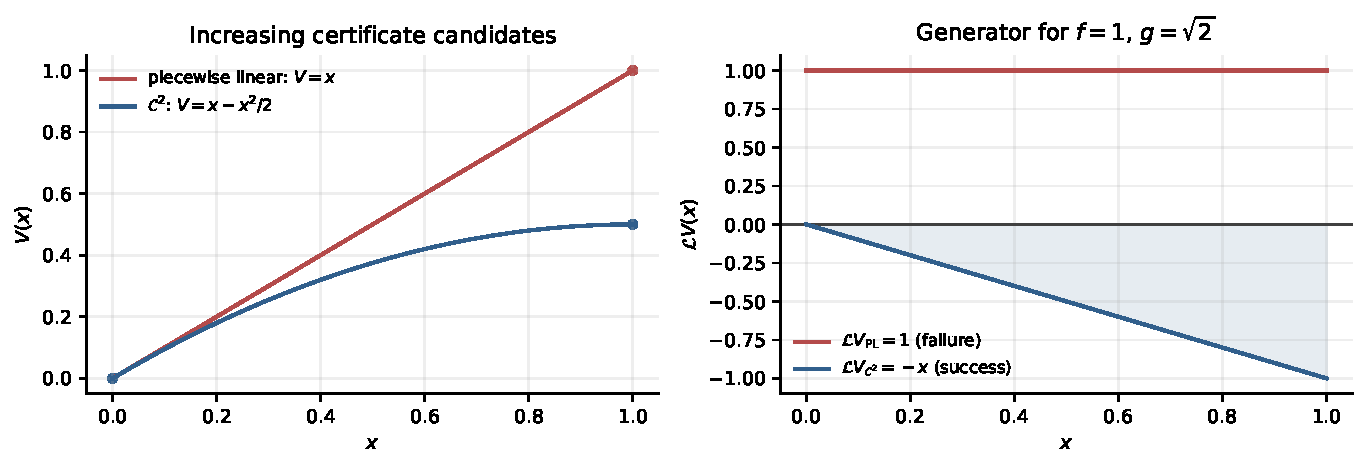
\includegraphics[width=\textwidth]{figures/linear_failure_curvature_success.pdf}
  \caption{An increasing piecewise-linear candidate fails the generator
  condition for $f=1$, $g=\sqrt{2}$, whereas negative curvature makes the
  smooth candidate satisfy it throughout $[0,1]$.}
  \label{fig:linear-vs-curved}
\end{figure}



\subsection{A piecewise $\mathcal{C}^2$ certificate with curvature and a kink}

Finally, let $dX_t=dW_t$ and
\[
  V(x)=
  \begin{cases}
    -\frac12x^2, & x<0,\\
    -x, & x\geq0.
  \end{cases}
\]
Here $D_t=0$, while
\[
  M_t=\int_0^t V'(X_s)\,dW_s,
  \qquad
  C_t=-\frac12\int_0^t\mathbf{1}_{\{X_s<0\}}\,ds,
  \qquad
  K_t=-\frac12L_t^0(X).
\]
Thus $C_t$ decreases while the path lies below zero, and $K_t$ decreases only
when local time accumulates at the kink. Figure~\ref{fig:hybrid-terms} shows
these different mechanisms on the same Brownian realization. The plotted
local time uses an occupation-density approximation with bandwidth $0.06$.

\begin{figure}[htbp]
  \centering
  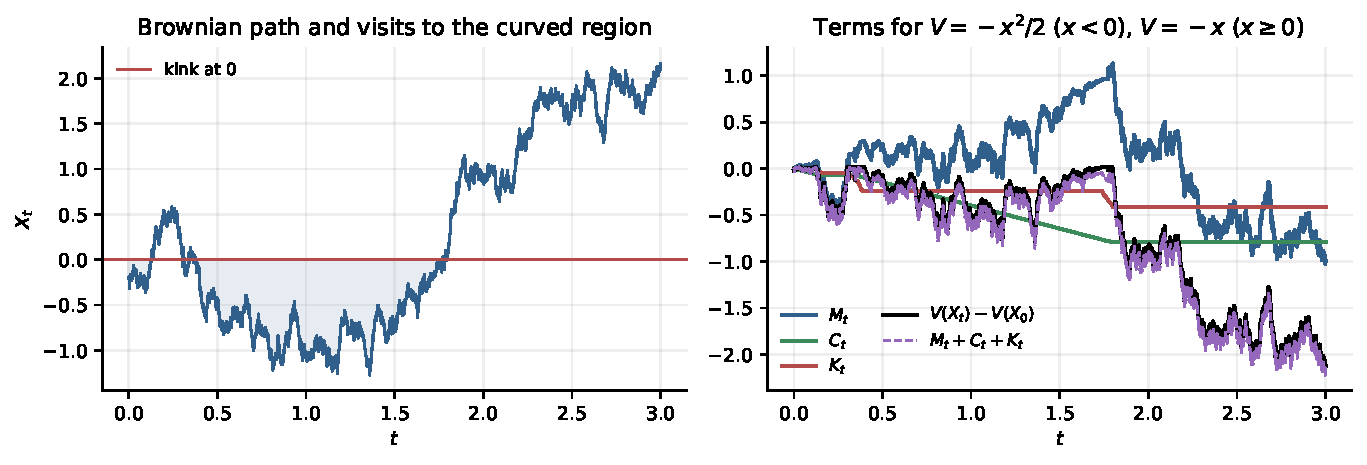
\includegraphics[width=\textwidth]{figures/hybrid_piecewise_c2_terms.pdf}
  \caption{A Brownian realization and the terms for the hybrid piecewise
  $\mathcal C^2$ certificate. The curvature and kink terms are both
  nonincreasing, while the martingale term fluctuates.}
  \label{fig:hybrid-terms}
\end{figure}

\newpage


\section{Piecewise quadratic certificates in dimension one}
\label{sec:piecewise-quadratic}

In this section, we will study a failure regime of the piecewise
linear certificates in dimension one and see how it leads to sufficiency
of piecewise quadratic certificates.

Additionally, we observe an interesting connection to the \textit{Taylor expansion} of the best possible
certificate, namely a martingale certificate for which the generator is zero.

\subsection{Failure of piecewise linear certificates in dimension one}

We will consider the setup from \autoref{sec:piecewise-linear} again, but with
additional assumptions on absorption at the boundary, an increase condition on
the piecewise linear function $V(x)$, and a non-degeneracy condition on the
diffusion term $g(x)$.

The key point is that the piecewise linear setup is not flexible enough when
the certificate is required to increase in the same direction as the drift. In
that case, a piecewise linear function has no curvature term which could
compensate for the positive drift contribution.

So essentially, we will show that:
\begin{fact}
(\textit{Informally.}) There is a case where no piecewise linear certificate can make $V(X_t)$ a
supermartingale.
\end{fact}

Although it should be clear from previous sections, for completeness, the setup
is as follows:

\begin{setup}
Let:
    \begin{enumerate}
        \item $dX_t = f(X_t)dt + g(X_t)dW_t$ be a one-dimensional SDE.
        \item $V(x)$ be a piecewise linear function such that
        $V(x)=a_i x+b_i$, where $x\in(x_i,x_{i+1})$.
        \item $V(x)$ is continuous at breakpoints:
        $V(x_i^+)=V(x_i^-)=V(x_i)$.
        \item as a consequence, $V'_{-}(x_i) = a_{i-1}$, $V'_{+}(x_i) = a_i$
        \item The $X_t$ process is \textbf{absorbed} at the boundary of
        $I=[a,b]$.
        \item $V(x)$ has the \textbf{increase condition} at the boundary:
        \begin{equation}
        V(a)<V(b).
        \end{equation}
        \item $g(x)^2>0$ for all $x\in(a,b)$, i.e. the \textbf{diffusion term is
        non-degenerate}.
        \item $M_t$ is a martingale, i.e. the \textbf{martingale condition}.
        \end{enumerate}
\end{setup}

Motivated by the example given in \autoref{sec:failure-of-piecewise-linear},
we will now show that there is a broad class of SDEs for which increasing
piecewise linear certificates cannot be supermartingales.

\begin{fact}
Assume that for all $\varepsilon>0$, there exists
$x\in(a,a+\varepsilon)$ such that
\begin{equation}
f(x)>0.
\label{eq:positive-drift-arbitrarily-close}
\end{equation}
Then there is no continuous piecewise linear $V$ satisfying the increase
condition
\begin{equation}
V(a)<V(b)
\end{equation}
and the concavity condition
\begin{equation}
V'_{+}(x_i)-V'_{-}(x_i)\leq 0
\end{equation}
at every breakpoint, such that $V(X_t)$ is a supermartingale.

\textbf{Proof}. Assume, for contradiction, that such a piecewise linear function $V$ exists
and that $V(X_t)$ is a supermartingale.

Let $p(x)=V'(x)$ on each linear region. Since $V$ is piecewise linear, the
Itô--Tanaka formula gives
\begin{align}
    V(X_t)
    &=
    V(X_0)
    +
    \int_0^t p(X_s)f(X_s)\,ds                                      \\
    &\quad
    +
    \int_0^t p(X_s)g(X_s)\,dW_s                                    \\
    &\quad
    +
    \frac12\sum_i
    \left(V'_+(x_i)-V'_-(x_i)\right)L_t^{x_i}(X).
\end{align}
The stochastic integral is a martingale by assumption. Therefore, if
$V(X_t)$ is a supermartingale, the finite-variation part cannot create
positive drift on any linear region. Hence the necessary interior condition
is
\begin{equation}
    p(x)f(x)\leq 0
    \qquad
    \text{on every linear region.}
    \label{eq:necessary-interior-condition-pl}
\end{equation}

This also follows from \hyperref[fact:nonpositive-drift-supermartingale]
  {Fact~\ref*{fact:nonpositive-drift-supermartingale}}
in \autoref{sec:piecewise-linear}.

We now use the concavity condition. Since
\begin{equation}
    V'_+(x_i)-V'_-(x_i)\leq 0
\end{equation}
at every breakpoint, the slopes of $V$ are nonincreasing from left to
right. Therefore $V$ is concave.

Let $(a,x_1)$ be the first linear region. We claim that the slope of $V$ on
this first region must be positive. Indeed, suppose instead that the first
slope were nonpositive. Since the slopes are nonincreasing, all later
slopes would also be nonpositive. Thus,
\begin{align}
    V(b)-V(a)
    &=
    \int_a^b V'(x)\,dx                                             \\
    &\leq 0.
\end{align}
This contradicts the increase condition $V(a)<V(b)$. Hence the first slope
must be positive, so
\begin{equation}
    p(x)>0
    \qquad
    \text{for all }x\in(a,x_1).
    \label{eq:first-slope-positive-pl}
\end{equation}

Now use the assumption on the drift. Since for every $\varepsilon>0$ there
exists $x\in(a,a+\varepsilon)$ such that $f(x)>0$, we may choose
$\varepsilon=x_1-a$. Then there exists $x^\ast\in(a,x_1)$ such that
\begin{equation}
    f(x^\ast)>0.
\end{equation}
Combining this with \eqref{eq:first-slope-positive-pl}, we get
\begin{equation}
    p(x^\ast)f(x^\ast)>0.
\end{equation}
This contradicts the necessary interior condition
\eqref{eq:necessary-interior-condition-pl}. Therefore no such piecewise
linear $V$ can make $V(X_t)$ a supermartingale.

\end{fact}

The conclusion is that piecewise linear certificates fail when the certificate
is forced to increase in the same direction as the drift. The obstruction comes
from the fact that piecewise linear functions have no interior curvature term.
Indeed, away from the kinks,
\begin{equation}
\mathcal L V(x)=V'(x)f(x),
\end{equation}
so a positive drift contribution cannot be compensated. This motivates the
piecewise quadratic case, where the additional curvature term
\begin{equation}
\frac12 V''(x)g(x)^2
\end{equation}
can offset the positive drift contribution.

\subsection{Sufficiency of piecewise quadratic certificates in dimension one}

In this subsection we will show that piecewise quadratic certificates are sufficient 
to guarantee that $V(X_t)$ is a supermartingale. 

Let $V$ be piecewise quadratic on $I=[a,b]$, so that on every interval
$(x_i,x_{i+1})$ we have
\begin{equation}
    V(x)=a_ i x^2+ b_i x+ c_i .
\end{equation}
Assume also that $V$ is continuous at the breakpoints. Then
\begin{equation}
    V'(x)=2a_i x+b_i,
    \qquad
    V''(x)=2a_i,
    \qquad x\in(x_i,x_{i+1}).
\end{equation}
Therefore the generator on the interior of a quadratic piece is
\begin{equation}
    \mathcal L V(x)
    =
    \left(2a_i x+b_i\right)f(x)
    +
    a_i g(x)^2.
    \label{eq:piecewise-quadratic-generator}
\end{equation}

Here, there are always exists a solution $(a_i,b_i)$ to the interior condition $\mathcal L V(x)\leq 0$ on each piece.

This gives the following sufficient condition.

\begin{fact}
Let $V$ be continuous and piecewise quadratic on $I=[a,b]$. Suppose that:
\begin{enumerate}
    \item on every open piece $(x_i,x_{i+1})$,
    \begin{equation}
        \mathcal L V(x)
        =
        V'(x)f(x)+\frac12 V''(x)g(x)^2
        \leq 0;
        \label{eq:pq-interior-condition}
    \end{equation}
    \item at every breakpoint,
    \begin{equation}
        V'_+(x_i)-V'_-(x_i)\leq 0;
        \label{eq:pq-kink-condition}
    \end{equation}
    \item the stochastic integral
    \begin{equation}
        M_t=\int_0^t V'(X_s)g(X_s)\,dW_s
    \end{equation}
    is a martingale.
\end{enumerate}
Then $V(X_t)$ is a supermartingale.

\textbf{Proof}. By the Itô--Tanaka formula for a piecewise $C^2$ function,
\begin{align}
    V(X_t)
    &=
    V(X_0)
    +
    \int_0^t
    \left(
        V'(X_s)f(X_s)+\frac12 V''(X_s)g(X_s)^2
    \right)ds                                                   \\
    &\quad+
    \int_0^t V'(X_s)g(X_s)\,dW_s                                \\
    &\quad+
    \frac12\sum_i
    \left(V'_+(x_i)-V'_-(x_i)\right)L_t^{x_i}(X).
\end{align}
The first term is nonincreasing by
\eqref{eq:pq-interior-condition}. The stochastic integral is a martingale by
assumption. Finally, since local time is nondecreasing in $t$, the kink term is
nonincreasing by \eqref{eq:pq-kink-condition}. 
Therefore $V(X_t)$ is a supermartingale.
\end{fact}

\subsection{Connection to Taylor expansion of the best possible certificate}

Let us now again consider the SDE
\begin{equation}
    dX_t=dt+\sqrt 2\,dW_t,
\end{equation}
the generator is
\begin{equation}
    \mathcal L V(x)=V'(x)+V''(x).
\end{equation}
A martingale certificate is obtained by asking for the generator to vanish:
\begin{equation}
    V'(x)+V''(x)=0.
    \label{eq:martingale-certificate-ode}
\end{equation}
Solving this ODE gives
\begin{equation}
    V(x)=C_1+C_2 e^{-x}.
\end{equation}
If we impose the normalization $V(0)=0$ and $V(1)=1$, then
\begin{equation}
    V_\star(x)
    =
    \frac{1-e^{-x}}{1-e^{-1}}.
    \label{eq:best-certificate-exp}
\end{equation}
This is the martingale certificate: $\mathcal L V_\star(x)=0$ on the interior.

Now expand the numerator of \eqref{eq:best-certificate-exp} around $0$:
\begin{equation}
    1-e^{-x}
    =
    x-\frac{x^2}{2}+\frac{x^3}{6}-\cdots .
\end{equation}
The quadratic certificate used above is exactly the second-order truncation of
this numerator:
\begin{equation}
    V_{\mathrm{quad}}(x)
    =
    x-\frac{x^2}{2}.
\end{equation}
So, up to the constant $(1-e^{-1})^{-1}$ and up to truncation
error, the quadratic certificate is the Taylor approximation of the martingale
certificate.

\section{Piecewise quadratic supermartingales in multiple dimensions}

Now we will finally consider a very general setup. 

First, we prove that when a piecewise-quadratic function $V : \mathbb{R}^d \to \mathbb{R}$ 
satisfies similar concativity and smoothness conditions as in the one-dimensional case, then $V(X_t)$ is a supermartingale.

Second, we will prove that if a smooth certificate exists, then we can construct a piecewise quadratic certificate that is a supermartingale,
essentially showing how quadratic certificates are in some sense sufficient, while piecewise linear certificates are not.

\subsection{Proving the supermartingale property}

We will show that a piecewise quadratic function gives a supermartingale if:
\begin{enumerate}
\item the generator is nonpositive inside each region,
\item the stochastic integral is a martingale,
\item the normal derivative jumps in the correct direction across each
interface.
\end{enumerate}

\begin{setup}
Let:
\begin{enumerate}
\item $dX_t = f(X_t)dt + \sigma(X_t)dW_t$ be a $d$-dimensional SDE, where
$f:\mathbb{R}^d \to \mathbb{R}^d$ and
$\sigma:\mathbb{R}^d \to \mathbb{R}^{d \times m}$.
\item $W_t$ is an $m$-dimensional Brownian motion.
\item $a(x) = \sigma(x)\sigma(x)^\top$.
\item $K \subseteq \mathbb{R}^d$ is a compact set partitioned into finitely
many polyhedral cells:
\[
K = \bigcup_{i=1}^N K_i.
\]
\item $V:K \to \mathbb{R}$ is a continuous piecewise quadratic function such
that
\[
V(x) = V_i(x)
=
c_i + p_i^\top x + \frac{1}{2}x^\top Q_i x,
\qquad x \in K_i,
\]
where $Q_i = Q_i^\top$.
\item $V$ is continuous across interfaces:
\[
V_i(x) = V_j(x),
\qquad x \in K_i \cap K_j.
\]
\end{enumerate}
\end{setup}

Now we will consider what conditions on $V$ are sufficient to guarantee that
$V(X_t)$ is a supermartingale, at least up to the first exit time from $K$.

Define the stopping time
\[
\tau_K = \inf\{t \geq 0 : X_t \notin K\}.
\]

\begin{hypothesis}
Does a multidimensional analogue of concavity, together with an interior
generator condition, guarantee that
\[
V(X_{t \wedge \tau_K})
\]
is a supermartingale?
\end{hypothesis}

To answer this, we apply the multidimensional Itô--Tanaka formula to
$V(X_{t \wedge \tau_K})$.

On each cell $K_i$, we have
\[
\nabla V_i(x) = p_i + Q_i x,
\qquad
\nabla^2 V_i(x) = Q_i.
\]

Therefore, the infinitesimal generator of $V_i$ is
\[
\mathcal{L}V_i(x)
=
\nabla V_i(x) \cdot f(x)
+
\frac{1}{2}
\operatorname{tr}\!\left(a(x)\nabla^2 V_i(x)\right).
\]

Substituting the quadratic form gives
\[
\mathcal{L}V_i(x)
=
(p_i + Q_i x)\cdot f(x)
+
\frac{1}{2}\operatorname{tr}\!\left(a(x)Q_i\right).
\]

Now let $F_{ij} = K_i \cap K_j$ be a shared interface between two neighbouring
cells. Let $n_{ij}$ be the unit normal vector pointing from $K_i$ into $K_j$.

The multidimensional Itô--Tanaka formula gives
\begin{align}
V(X_{t \wedge \tau_K})
=
V(X_0)
&+
\int_0^{t \wedge \tau_K}
\mathcal{L}V(X_s) ds \\
&+
\int_0^{t \wedge \tau_K}
\nabla V(X_s)^\top \sigma(X_s) dW_s \\
&+
\frac{1}{2}
\sum_{i<j}
\int_0^{t \wedge \tau_K}
\left(
\nabla V_j(X_s) - \nabla V_i(X_s)
\right)\cdot n_{ij}
dL_s^{F_{ij}} .
\end{align}

Here $L_t^{F_{ij}}$ denotes the surface local time accumulated by $X_t$ on the
interface $F_{ij}$.

We will focus on these terms:

\begin{enumerate}
\item
\[
D_t
=
\int_0^{t \wedge \tau_K}
\mathcal{L}V(X_s)ds,
\]
the interior drift term.

\item
\[
    M_t
    =
    \int_0^{t \wedge \tau_K}
    \nabla V(X_s)^\top \sigma(X_s)dW_s,
\]
the diffusion term.

\item
\[
    K_t
    =
    \frac{1}{2}
    \sum_{i<j}
    \int_0^{t \wedge \tau_K}
    \left(
        \nabla V_j(X_s) - \nabla V_i(X_s)
    \right)\cdot n_{ij}
    dL_s^{F_{ij}},
\]
the interface term.
\end{enumerate}

We need to prove that
\[
D_t + M_t + K_t
\]
is a supermartingale.

Some natural assumptions, which are sufficient to guarantee that
$V(X_{t \wedge \tau_K})$ is a supermartingale, are the following.

\begin{enumerate}
\item
The interior generator is nonpositive on every cell:
\[
\mathcal{L}V_i(x) \leq 0,
\qquad x \in \operatorname{int}(K_i).
\]
Equivalently,
\[
(p_i + Q_i x)\cdot f(x)
+
\frac{1}{2}\operatorname{tr}\!\left(a(x)Q_i\right)
\leq 0,
\qquad x \in \operatorname{int}(K_i).
\]

This is the multidimensional analogue of the condition
\[
    f(x)V'(x) \leq 0
\]
from the one-dimensional piecewise linear case.

\begin{fact}
If $\mathcal{L}V(X_s) \leq 0$ for all $s \leq \tau_K$, then the drift term
$D_t$ is a supermartingale.

\textbf{Proof:} We want to prove
\[
    \mathbb{E}[D_t \mid \mathcal{F}_r] \leq D_r,
    \qquad r \leq t.
\]
By definition,
\begin{align}
    \mathbb{E}[D_t \mid \mathcal{F}_r]
    &=
    \mathbb{E}\left[
    \int_0^{t \wedge \tau_K}
    \mathcal{L}V(X_s)ds
    \Bigm| \mathcal{F}_r
    \right] \\
    &=
    \int_0^{r \wedge \tau_K}
    \mathcal{L}V(X_s)ds
    +
    \mathbb{E}\left[
    \int_{r \wedge \tau_K}^{t \wedge \tau_K}
    \mathcal{L}V(X_s)ds
    \Bigm| \mathcal{F}_r
    \right].
\end{align}
Since $\mathcal{L}V(X_s) \leq 0$, the second term is nonpositive. Hence
\[
    \mathbb{E}[D_t \mid \mathcal{F}_r]
    \leq
    D_r.
\]
Therefore $D_t$ is a supermartingale.
\end{fact}

\item
The stochastic integral $M_t$ is a martingale. A sufficient condition is
\[
    \mathbb{E}\left[
    \int_0^{t \wedge \tau_K}
    \left\|
        \nabla V(X_s)^\top \sigma(X_s)
    \right\|^2 ds
    \right]
    < \infty.
\]
Since $V$ is piecewise quadratic on finitely many cells, $\nabla V$ is
piecewise linear. Therefore, on a compact set $K$, $\nabla V$ is bounded.
Thus this condition is usually easy to verify if $\sigma$ is bounded on $K$.

\item
The interface contribution is nonpositive. For every shared face
\[
    F_{ij} = K_i \cap K_j,
\]
we assume
\[
    \left(
        \nabla V_j(x) - \nabla V_i(x)
    \right)\cdot n_{ij}
    \leq 0,
    \qquad x \in F_{ij}.
\]
Since
\[
    \nabla V_i(x) = p_i + Q_i x
\]
and
\[
    \nabla V_j(x) = p_j + Q_j x,
\]
this condition can be written explicitly as
\[
    \left(
        p_j - p_i + (Q_j - Q_i)x
    \right)\cdot n_{ij}
    \leq 0,
    \qquad x \in F_{ij}.
\]

This is the multidimensional version of the concavity condition
\[
    V'_+(x_i) - V'_-(x_i) \leq 0
\]
from the one-dimensional case.

\begin{fact}
If
\[
    \left(
        \nabla V_j(x) - \nabla V_i(x)
    \right)\cdot n_{ij}
    \leq 0
    \qquad \text{on } F_{ij},
\]
and $L_t^{F_{ij}}$ is nondecreasing in $t$, then the interface term $K_t$ is
a supermartingale.

\textbf{Proof:} We want to prove
\[
    \mathbb{E}[K_t \mid \mathcal{F}_r] \leq K_r,
    \qquad r \leq t.
\]
The interface term is
\[
    K_t
    =
    \frac{1}{2}
    \sum_{i<j}
    \int_0^{t \wedge \tau_K}
    \gamma_{ij}(X_s)dL_s^{F_{ij}},
\]
where
\[
    \gamma_{ij}(x)
    =
    \left(
        \nabla V_j(x) - \nabla V_i(x)
    \right)\cdot n_{ij}.
\]
By assumption,
\[
    \gamma_{ij}(x) \leq 0
    \qquad x \in F_{ij}.
\]
Also, $dL_s^{F_{ij}}$ is a nonnegative measure, because surface local time is
nondecreasing. Therefore
\[
    \int_r^t \gamma_{ij}(X_s)dL_s^{F_{ij}} \leq 0.
\]
Hence the future increment of $K_t$ after time $r$ is nonpositive, and so
\[
    \mathbb{E}[K_t \mid \mathcal{F}_r] \leq K_r.
\]
Therefore $K_t$ is a supermartingale.
\end{fact}
\end{enumerate}

\subsubsection{Proof of the supermartingale property}

We now combine the three conditions.

By the multidimensional Itô--Tanaka formula,
\begin{align}
V(X_{t \wedge \tau_K})
=
V(X_0)
+
D_t
+
M_t
+
K_t.
\end{align}

The drift term $D_t$ is a supermartingale by the interior generator condition:
\[
\mathcal{L}V_i(x) \leq 0
\qquad x \in \operatorname{int}(K_i).
\]

The stochastic integral $M_t$ is a martingale by the square-integrability
assumption:
\[
\mathbb{E}\left[
\int_0^{t \wedge \tau_K}
\left|
\nabla V(X_s)^\top \sigma(X_s)
\right|^2 ds
\right]
< \infty.
\]

The interface term $K_t$ is a supermartingale by the multidimensional concavity
condition:
\[
\left(
\nabla V_j(x) - \nabla V_i(x)
\right)\cdot n_{ij}
\leq 0,
\qquad x \in F_{ij}.
\]

Therefore $D_t + K_t$ is a supermartingale, and $M_t$ is a martingale. Since the
sum of a martingale and a supermartingale is a supermartingale, we conclude that
\[
V(X_{t \wedge \tau_K})
\]
is a supermartingale.

\subsubsection{Interpretation of the multidimensional concavity condition}

The condition
\[
\left(
\nabla V_j(x) - \nabla V_i(x)
\right)\cdot n_{ij}
\leq 0,
\qquad x \in F_{ij},
\]
says that when the process crosses from cell $K_i$ into cell $K_j$, the
directional derivative of $V$ in the crossing direction cannot increase.

Indeed, the normal derivative from the $K_i$ side is
\[
\nabla V_i(x)\cdot n_{ij},
\]
while the normal derivative from the $K_j$ side is
\[
\nabla V_j(x)\cdot n_{ij}.
\]

Thus the condition is equivalent to
\[
\nabla V_j(x)\cdot n_{ij}
\leq
\nabla V_i(x)\cdot n_{ij}.
\]

This is exactly the analogue of the one-dimensional condition
\[
V'_+(x_i) \leq V'_-(x_i).
\]

So, in multiple dimensions, ordinary concavity is not the only thing we need to
look at. What matters for the local time term is the jump in the normal
derivative across each interface. If that jump is nonpositive, then the surface
local time contribution pushes $V(X_t)$ downwards rather than upwards.

\subsubsection{Summary of sufficient conditions}

We have shown that the following assumptions are sufficient.

\begin{enumerate}
\item $V$ is continuous and piecewise quadratic:
\[
V(x)
=
c_i + p_i^\top x + \frac{1}{2}x^\top Q_i x,
\qquad x \in K_i.
\]

\item The generator is nonpositive inside each cell:
\[
    (p_i + Q_i x)\cdot f(x)
    +
    \frac{1}{2}\operatorname{tr}\!\left(a(x)Q_i\right)
    \leq 0,
    \qquad x \in \operatorname{int}(K_i).
\]

\item The stochastic integral is a martingale:
\[
    \mathbb{E}\left[
    \int_0^{t \wedge \tau_K}
    \left\|
        \nabla V(X_s)^\top \sigma(X_s)
    \right\|^2 ds
    \right]
    < \infty.
\]

\item The interface condition holds on every shared face:
\[
    \left(
        p_j - p_i + (Q_j - Q_i)x
    \right)\cdot n_{ij}
    \leq 0,
    \qquad x \in F_{ij}.
\]
\end{enumerate}

Under these assumptions,
\[
V(X_{t \wedge \tau_K})
\]
is a supermartingale.

This gives the multidimensional version of the one-dimensional piecewise linear
certificate result. The interior generator condition controls the ordinary Itô
drift, while the interface concavity condition controls the Tanaka local time
terms.

\subsection{Asymptotic completeness of piecewise quadratic certificates}

\paragraph{Theorem (asymptotic completeness under a strict smooth certificate).}
Let \(K\subset\mathbb R^2\) be compact and polygonal, and consider the stopped
SDE
\[
  dX_t=f(X_t)\,dt+\sigma(X_t)\,dW_t,
  \qquad
  a(x)=\sigma(x)\sigma(x)^\top,
\]
stopped at
\[
  \tau_K=\inf\{t\ge0:X_t\notin K\}.
\]
Assume that \(f\) and \(a\) are bounded on \(K\).  Suppose there exists a
strict smooth certificate \(U\in C^3(K)\) such that
\[
  \mathcal LU(x)
  =
  \nabla U(x)\cdot f(x)
  +
  \frac12\operatorname{tr}\!\bigl(a(x)\nabla^2U(x)\bigr)
  \le -\varepsilon
  \qquad x\in K,
\]
for some \(\varepsilon>0\).  Assume also that the boundary/separation
conditions hold with margin: for some \(\delta>0\),
\[
  \sup_{x\in X_0}U(x)\le \alpha-\delta,
  \qquad
  \inf_{x\in X_u}U(x)\ge \beta+\delta,
  \qquad
  \alpha<\beta.
\]

Let \(\{\mathcal T_h\}_{h\downarrow0}\) be a shape-regular sequence of
refined triangulations of \(K\) supporting \(C^1\) piecewise-quadratic spline
interpolants \(I_hU\) satisfying
\[
  \|I_hU-U\|_{C^2(K)}\to0
  \qquad\text{as }h\to0.
\]
Then, for all sufficiently small \(h\), the function
\[
  V_h:=I_hU
\]
is a continuous \(C^1\) piecewise-quadratic certificate satisfying
\[
  \mathcal LV_h(x)\le -\frac{\varepsilon}{2}
  \qquad x\in K,
\]
and
\[
  \sup_{x\in X_0}V_h(x)\le \alpha,
  \qquad
  \inf_{x\in X_u}V_h(x)\ge \beta.
\]
Consequently,
\[
  V_h(X_{t\wedge\tau_K})
\]
is a supermartingale.

\paragraph{Proof.}
Since \(f\) and \(a\) are bounded on \(K\), define
\[
  F:=\sup_{x\in K}\|f(x)\|,
  \qquad
  A:=\sup_{x\in K}\|a(x)\|.
\]
Let
\[
  E_h:=V_h-U.
\]
Then
\[
  \mathcal LV_h-\mathcal LU
  =
  \nabla E_h\cdot f
  +
  \frac12\operatorname{tr}\!\bigl(a\nabla^2E_h\bigr).
\]
Hence, for a constant \(C_K>0\) depending only on the dimension and the chosen
matrix norm,
\[
  |\mathcal LV_h(x)-\mathcal LU(x)|
  \le
  F\|\nabla E_h\|_{L^\infty(K)}
  +
  C_K A\|\nabla^2E_h\|_{L^\infty(K)}.
\]
Because
\[
  \|E_h\|_{C^2(K)}\to0,
\]
there exists \(h_0>0\) such that, for all \(h<h_0\),
\[
  |\mathcal LV_h(x)-\mathcal LU(x)|
  \le \frac{\varepsilon}{2}
  \qquad x\in K.
\]
Since \(\mathcal LU\le-\varepsilon\), it follows that
\[
  \mathcal LV_h
  \le
  -\varepsilon+\frac{\varepsilon}{2}
  =
  -\frac{\varepsilon}{2}.
\]

Similarly, since \(V_h\to U\) uniformly, for all sufficiently small \(h\),
\[
  \|V_h-U\|_{L^\infty(K)}\le\delta.
\]
Therefore
\[
  \sup_{X_0}V_h
  \le
  \sup_{X_0}U+\delta
  \le
  \alpha,
\]
and
\[
  \inf_{X_u}V_h
  \ge
  \inf_{X_u}U-\delta
  \ge
  \beta.
\]

It remains to check the nonsmooth interfaces.  The spline \(V_h\) is
\(C^1\) across every internal face of the triangulation.  Therefore, if two
quadratic pieces \(V_i,V_j\) meet across a face \(F_{ij}\), then
\[
  \nabla V_i(x)=\nabla V_j(x)
  \qquad x\in F_{ij}.
\]
Hence the Tanaka normal-derivative jump is
\[
  \bigl[\nabla V_j(x)-\nabla V_i(x)\bigr]\cdot n_{i\to j}=0,
\]
so every local-time contribution is zero.

Applying the multidimensional It\^o--Tanaka formula gives
\[
  V_h(X_{t\wedge\tau_K})
  =
  V_h(X_0)
  +
  \int_0^{t\wedge\tau_K}\mathcal LV_h(X_s)\,ds
  +
  \int_0^{t\wedge\tau_K}\nabla V_h(X_s)\sigma(X_s)\,dW_s.
\]
The drift term is nonpositive because
\[
  \mathcal LV_h\le-\frac{\varepsilon}{2}<0.
\]
The stochastic integral is a true martingale after stopping, since \(K\) is
compact and \(V_h,\sigma\) are bounded on \(K\).  Therefore
\[
  V_h(X_{t\wedge\tau_K})
\]
is a martingale plus a nonincreasing finite-variation process, and is hence a
supermartingale. \(\square\)


\end{document}
